\documentclass{article}
\usepackage[utf8]{inputenc}
\usepackage[top=0.75in, bottom=0.75in, left=0.65in, right=0.65in]{geometry}
\usepackage{graphicx}
\usepackage{amsmath}
\usepackage{amsmath}
\usepackage{amssymb}
\usepackage{listings}
\usepackage[T1]{fontenc}
\usepackage[lighttt]{lmodern}

\usepackage{xcolor}
 
\definecolor{codegreen}{rgb}{0,0.6,0}
\definecolor{codegray}{rgb}{0.5,0.5,0.5}
\definecolor{codepurple}{rgb}{0.58,0,0.82}
\definecolor{backcolour}{rgb}{0.95,0.95,0.92}
 
\lstdefinestyle{mystyle}{
    backgroundcolor=\color{white},   
    commentstyle=\color{codegreen},
    keywordstyle=\color{magenta},
    numberstyle=\tiny\color{codegray},
    stringstyle=\color{codepurple},
    basicstyle=\ttfamily\footnotesize,
    breakatwhitespace=false,         
    breaklines=true,                 
    captionpos=b,                    
    keepspaces=true,                 
    numbers=left,                    
    numbersep=5pt,                  
    showspaces=false,                
    showstringspaces=false,
    showtabs=false,                  
    tabsize=2
}

\lstset{style=mystyle}
\usepackage{graphicx}
\graphicspath{{figure/}}


\newcommand*\lstinputpath[1]{\lstset{inputpath=#1}}
\lstinputpath{codes}
\title{Home Work 01: EAS 520}
\author{Sayem Khan}
\date{Tuesday, October 8, 2019}

\begin{document}

\maketitle

\subsubsection*{Problem a} 
Specialize the general Monte Carlo integration method.
\subsubsection*{Solution}
The problem is,
\begin{equation}
   I_1 = \int_{-1}^{1}\frac{1}{1+x^2}dx
   \label{one}
\end{equation}
We need to write equation (\ref{one}) as 1-D Monte Carlo integration formula, that is,
\begin{equation}
   \hat{I}_{N} = V\frac{1}{N}\sum_{i = 1}^{N}\frac{1}{1+x_i^2} =2\frac{1}{N}\sum_{i = 1}^{N}\frac{1}{1+x_i^2}
   \label{two}
\end{equation}
where, $N\to \infty $, each $x_i$ is randomly and uniformly drawn from the interval $\left [ -1,1 \right ]$ and $V$ is the \textit{volume}, that is in this case,
\begin{equation*}
  V = \int_{-1}^{1}dx = x\mid^{1}_{-1} = 1-(-1) = 2
\end{equation*}
\subsubsection*{Problem b } 
The Pseudocode to compute the integration of equation \ref{two}. 
\subsubsection*{Solution}
\lstinputlisting[
  language   = python,
  basicstyle = \ttfamily,
  frame      = single,
  caption    = {Pseudocode for equation \ref{two}},
]{mcAlgo.py}

\subsubsection*{Problem c } 
\subsubsection*{Solution}
The implementation of equation \ref{two} in C++ given below:
\lstinputlisting[
  language = C++,
  basicstyle = \ttfamily,
  frame      = single,
  caption    = {\textbf{monteCarlo.cpp}:  C++ implementation for equation (\ref{two}) with error calculation.},
]{monteCarlo.cpp}
\vspace{13mm}
The bash script for Problem d, e, f given below:
\lstinputlisting[
  language = bash,
  basicstyle = \ttfamily,
  frame      = single,
  caption    = {Bash script \textbf{dataScript.sh} for execution and data generation in Problem d, e, f },
]{dataScript.sh}

\subsubsection*{Problem d, e, f} 
\subsubsection*{Solution}
\begin{figure}[h!]
  \centering
    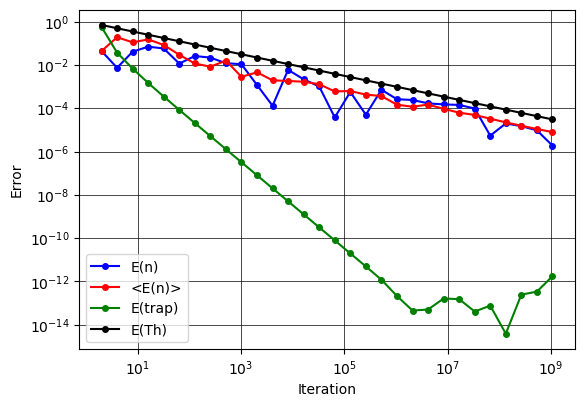
\includegraphics[width=0.85\textwidth]{Numerical_Intergration_Err_vs_Iteration.png}
    \caption{Numerical Integration Err vs Iteration: Problem d, e, f} 
    \label{EvsN}
\end{figure}
Here in the figure \ref{EvsN}, the Error vs Iteration is being plotted. The sequence of $N = 2^i$ for integers $i = 1, 2, 3,\cdots,30$ used as input. The theoretical error of the Monte Carlo integration is $E \propto N^{-1/2} $. \\
Here, the experiment run $200$ times and average error is being calculated.
\\
\\
\textbf{Problem e Solution:}
Here the error behaves like: 
$$
logE(N) = B + A\times log(N)
$$
If we assume $B = 0$ (since it is a constant), using the linear regression analysis, it is found that: 
$$A = -0.6049353724290725$$
But, it should be equal to $-0.5$. Since, several errors like rounding error and random number 
generation contributes error here. 
\subsubsection*{Problem g} 
\subsubsection*{Solution}
The execution time taken by \textbf{time.sh}.
\lstinputlisting[
  language = bash,
  basicstyle = \ttfamily,
  frame      = single,
  caption    = {\textbf{time.sh}: For execution and data generation in Problem g },
]{time.sh}
\begin{figure}[h!]
  \centering
    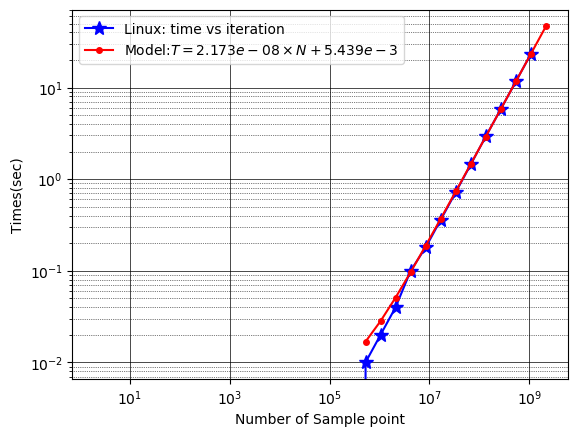
\includegraphics[width=0.9\textwidth]{Time_vs_Number_of_Sample_point_curve}
    \caption{Time vs Iteration: Problem g} 
    \label{time}
\end{figure}

The run time is calculated by the Linux \textit{time} command. For first $18$ iteration, we got zero (0). Perhaps, CPU take some time in 'nano' second scale. So, \textit{time} command ignored that. The time data is plotted in \ref{time}. We have seen that the relation between iteration and time is linear. From the data, the best fitted model for time is: 
$$
T = 2.17309336\times 10^{-8} \times N + 5.4391834667749 \times 10^{-3} 
$$
where, T is time in second and N is number of iteration. Using this formula as well as using linear regression, it is found that time for $N = 2^{32}$ is $93.339$ seconds.
$$$$
\end{document}
